% roofline.tex: generado por tools/p7/tablas.py (make p7-rapido). No editar a mano.
% Uso: % roofline.tex: generado por tools/p7/tablas.py (make p7-rapido). No editar a mano.
% Uso: % roofline.tex: generado por tools/p7/tablas.py (make p7-rapido). No editar a mano.
% Uso: % roofline.tex: generado por tools/p7/tablas.py (make p7-rapido). No editar a mano.
% Uso: \input{roofline.tex} dentro de una figura. Ejes en log10: x de 0,01 a 100 Op/B, y de 0,1 a 1000 MOPS.
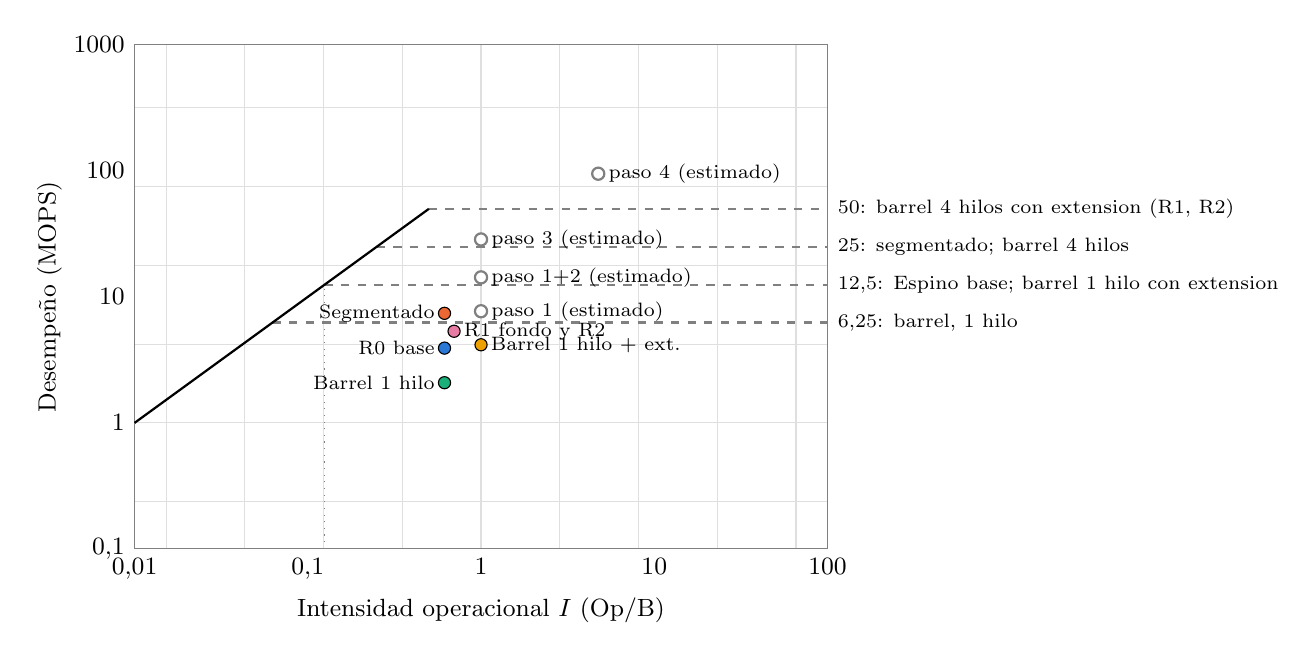
\begin{tikzpicture}[x=2.2cm,y=1.6cm,font=\small]
  \draw[gray!25] (-2,-1) grid (2,3);
  \draw[gray] (-2,-1) rectangle (2,3);
  \node[below] at (-2,-1) {$0{,}01$};
  \node[below] at (-1,-1) {$0{,}1$};
  \node[below] at (0,-1) {$1$};
  \node[below] at (1,-1) {$10$};
  \node[below] at (2,-1) {$100$};
  \node[left] at (-2,-1) {$0{,}1$};
  \node[left] at (-2,0) {$1$};
  \node[left] at (-2,1) {$10$};
  \node[left] at (-2,2) {$100$};
  \node[left] at (-2,3) {$1000$};
  \node[below=5mm] at (0.0,-1) {Intensidad operacional $I$ (Op/B)};
  \node[rotate=90,above=8mm] at (-2,1.0) {Desempeño (MOPS)};
  \draw[gray,dashed,thick] (-1.2041,0.7959) -- (2,0.7959) node[right,black,font=\scriptsize] {6{,}25: barrel{,} 1 hilo};
  \draw[gray,dashed,thick] (-0.9031,1.0969) -- (2,1.0969) node[right,black,font=\scriptsize] {12{,}5: Espino base; barrel 1 hilo con extension};
  \draw[gray,dashed,thick] (-0.6021,1.3979) -- (2,1.3979) node[right,black,font=\scriptsize] {25: segmentado; barrel 4 hilos};
  \draw[gray,dashed,thick] (-0.3010,1.6990) -- (2,1.6990) node[right,black,font=\scriptsize] {50: barrel 4 hilos con extension (R1{,} R2)};
  \draw[black,thick] (-2,0.0000) -- (-0.3010,1.6990);
  \draw[gray,dotted] (-0.9031,-1) -- (-0.9031,1.0969);
  \filldraw[fill={rgb,255:red,42;green,120;blue,214}] (-0.2108,0.5935) circle (2.2pt) node[left,font=\scriptsize,black] {R0 base};
  \filldraw[fill={rgb,255:red,235;green,104;blue,52}] (-0.2108,0.8697) circle (2.2pt) node[left,font=\scriptsize,black] {Segmentado};
  \filldraw[fill={rgb,255:red,27;green,175;blue,122}] (-0.2108,0.3188) circle (2.2pt) node[left,font=\scriptsize,black] {Barrel 1 hilo};
  \filldraw[fill={rgb,255:red,237;green,161;blue,0}] (0.0000,0.6198) circle (2.2pt) node[right,font=\scriptsize,black] {Barrel 1 hilo + ext.};
  \filldraw[fill={rgb,255:red,232;green,123;blue,164}] (-0.1556,0.7272) circle (2.2pt) node[right,font=\scriptsize,black] {R1 fondo y R2};
  \filldraw[draw=gray,thick,fill=white] (0.0000,0.8861) circle (2.2pt) node[right,font=\scriptsize,black] {paso 1 (estimado)};
  \filldraw[draw=gray,thick,fill=white] (0.0000,1.1549) circle (2.2pt) node[right,font=\scriptsize,black] {paso 1+2 (estimado)};
  \filldraw[draw=gray,thick,fill=white] (0.0000,1.4559) circle (2.2pt) node[right,font=\scriptsize,black] {paso 3 (estimado)};
  \filldraw[draw=gray,thick,fill=white] (0.6767,1.9777) circle (2.2pt) node[right,font=\scriptsize,black] {paso 4 (estimado)};
\end{tikzpicture}
 dentro de una figura. Ejes en log10: x de 0,01 a 100 Op/B, y de 0,1 a 1000 MOPS.
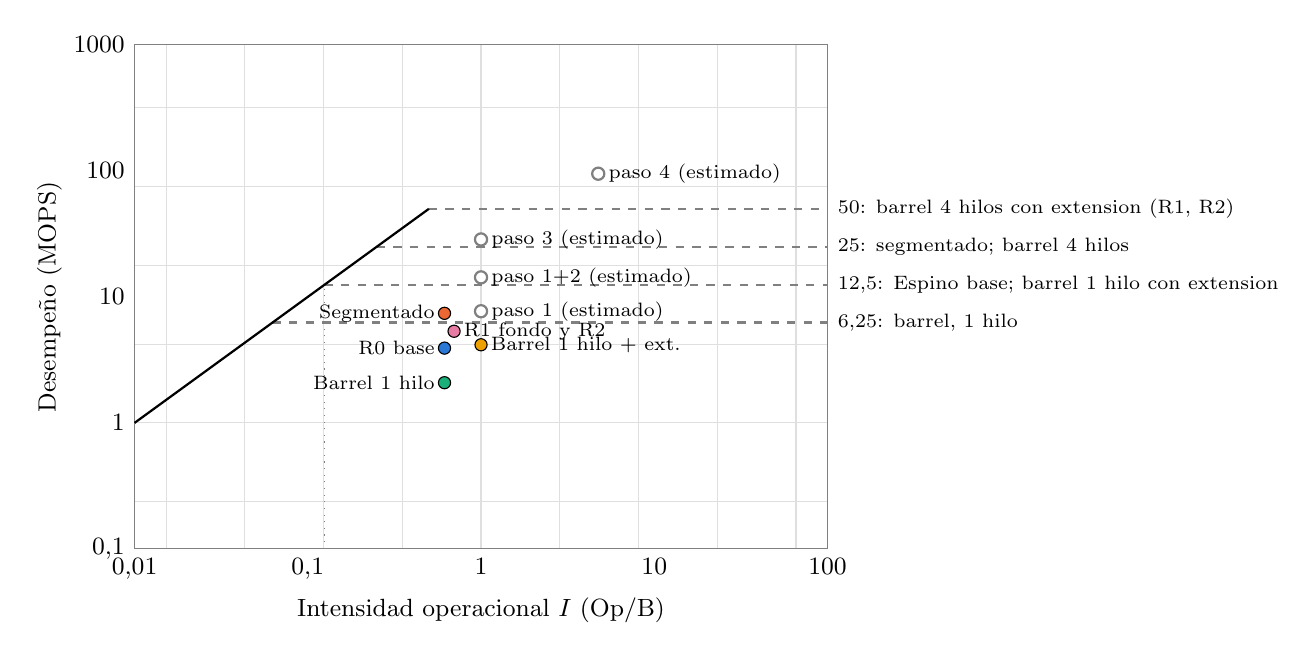
\begin{tikzpicture}[x=2.2cm,y=1.6cm,font=\small]
  \draw[gray!25] (-2,-1) grid (2,3);
  \draw[gray] (-2,-1) rectangle (2,3);
  \node[below] at (-2,-1) {$0{,}01$};
  \node[below] at (-1,-1) {$0{,}1$};
  \node[below] at (0,-1) {$1$};
  \node[below] at (1,-1) {$10$};
  \node[below] at (2,-1) {$100$};
  \node[left] at (-2,-1) {$0{,}1$};
  \node[left] at (-2,0) {$1$};
  \node[left] at (-2,1) {$10$};
  \node[left] at (-2,2) {$100$};
  \node[left] at (-2,3) {$1000$};
  \node[below=5mm] at (0.0,-1) {Intensidad operacional $I$ (Op/B)};
  \node[rotate=90,above=8mm] at (-2,1.0) {Desempeño (MOPS)};
  \draw[gray,dashed,thick] (-1.2041,0.7959) -- (2,0.7959) node[right,black,font=\scriptsize] {6{,}25: barrel{,} 1 hilo};
  \draw[gray,dashed,thick] (-0.9031,1.0969) -- (2,1.0969) node[right,black,font=\scriptsize] {12{,}5: Espino base; barrel 1 hilo con extension};
  \draw[gray,dashed,thick] (-0.6021,1.3979) -- (2,1.3979) node[right,black,font=\scriptsize] {25: segmentado; barrel 4 hilos};
  \draw[gray,dashed,thick] (-0.3010,1.6990) -- (2,1.6990) node[right,black,font=\scriptsize] {50: barrel 4 hilos con extension (R1{,} R2)};
  \draw[black,thick] (-2,0.0000) -- (-0.3010,1.6990);
  \draw[gray,dotted] (-0.9031,-1) -- (-0.9031,1.0969);
  \filldraw[fill={rgb,255:red,42;green,120;blue,214}] (-0.2108,0.5935) circle (2.2pt) node[left,font=\scriptsize,black] {R0 base};
  \filldraw[fill={rgb,255:red,235;green,104;blue,52}] (-0.2108,0.8697) circle (2.2pt) node[left,font=\scriptsize,black] {Segmentado};
  \filldraw[fill={rgb,255:red,27;green,175;blue,122}] (-0.2108,0.3188) circle (2.2pt) node[left,font=\scriptsize,black] {Barrel 1 hilo};
  \filldraw[fill={rgb,255:red,237;green,161;blue,0}] (0.0000,0.6198) circle (2.2pt) node[right,font=\scriptsize,black] {Barrel 1 hilo + ext.};
  \filldraw[fill={rgb,255:red,232;green,123;blue,164}] (-0.1556,0.7272) circle (2.2pt) node[right,font=\scriptsize,black] {R1 fondo y R2};
  \filldraw[draw=gray,thick,fill=white] (0.0000,0.8861) circle (2.2pt) node[right,font=\scriptsize,black] {paso 1 (estimado)};
  \filldraw[draw=gray,thick,fill=white] (0.0000,1.1549) circle (2.2pt) node[right,font=\scriptsize,black] {paso 1+2 (estimado)};
  \filldraw[draw=gray,thick,fill=white] (0.0000,1.4559) circle (2.2pt) node[right,font=\scriptsize,black] {paso 3 (estimado)};
  \filldraw[draw=gray,thick,fill=white] (0.6767,1.9777) circle (2.2pt) node[right,font=\scriptsize,black] {paso 4 (estimado)};
\end{tikzpicture}
 dentro de una figura. Ejes en log10: x de 0,01 a 100 Op/B, y de 0,1 a 1000 MOPS.
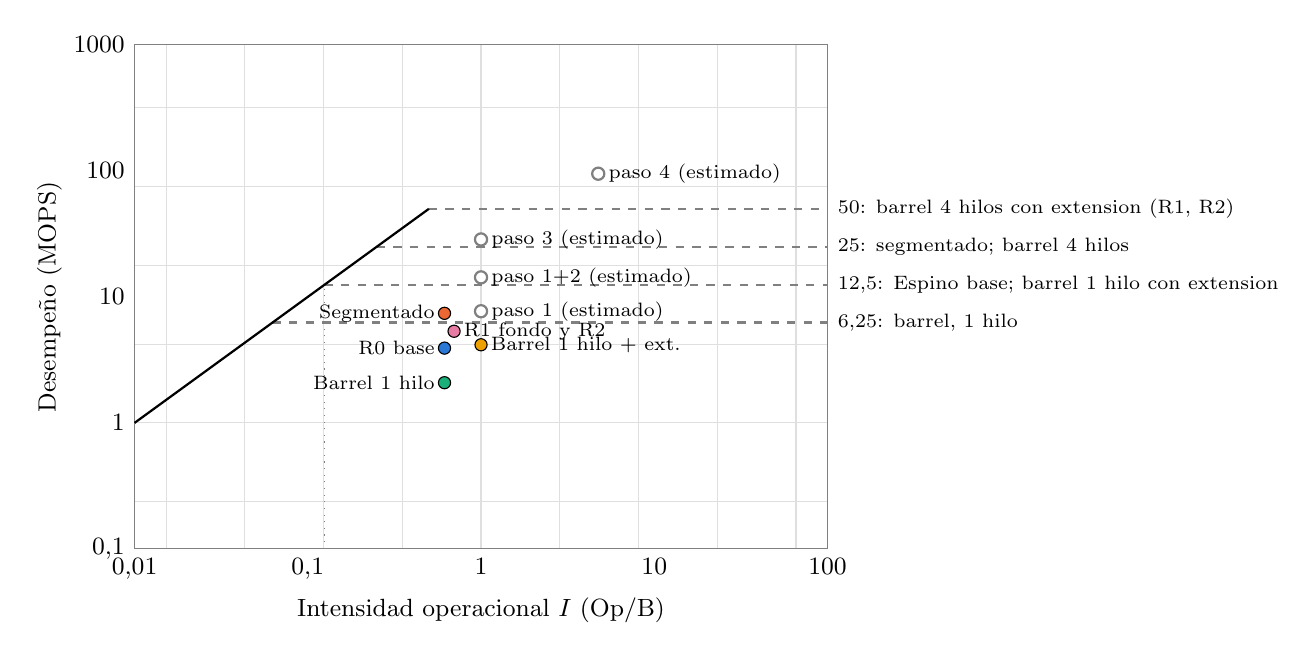
\begin{tikzpicture}[x=2.2cm,y=1.6cm,font=\small]
  \draw[gray!25] (-2,-1) grid (2,3);
  \draw[gray] (-2,-1) rectangle (2,3);
  \node[below] at (-2,-1) {$0{,}01$};
  \node[below] at (-1,-1) {$0{,}1$};
  \node[below] at (0,-1) {$1$};
  \node[below] at (1,-1) {$10$};
  \node[below] at (2,-1) {$100$};
  \node[left] at (-2,-1) {$0{,}1$};
  \node[left] at (-2,0) {$1$};
  \node[left] at (-2,1) {$10$};
  \node[left] at (-2,2) {$100$};
  \node[left] at (-2,3) {$1000$};
  \node[below=5mm] at (0.0,-1) {Intensidad operacional $I$ (Op/B)};
  \node[rotate=90,above=8mm] at (-2,1.0) {Desempeño (MOPS)};
  \draw[gray,dashed,thick] (-1.2041,0.7959) -- (2,0.7959) node[right,black,font=\scriptsize] {6{,}25: barrel{,} 1 hilo};
  \draw[gray,dashed,thick] (-0.9031,1.0969) -- (2,1.0969) node[right,black,font=\scriptsize] {12{,}5: Espino base; barrel 1 hilo con extension};
  \draw[gray,dashed,thick] (-0.6021,1.3979) -- (2,1.3979) node[right,black,font=\scriptsize] {25: segmentado; barrel 4 hilos};
  \draw[gray,dashed,thick] (-0.3010,1.6990) -- (2,1.6990) node[right,black,font=\scriptsize] {50: barrel 4 hilos con extension (R1{,} R2)};
  \draw[black,thick] (-2,0.0000) -- (-0.3010,1.6990);
  \draw[gray,dotted] (-0.9031,-1) -- (-0.9031,1.0969);
  \filldraw[fill={rgb,255:red,42;green,120;blue,214}] (-0.2108,0.5935) circle (2.2pt) node[left,font=\scriptsize,black] {R0 base};
  \filldraw[fill={rgb,255:red,235;green,104;blue,52}] (-0.2108,0.8697) circle (2.2pt) node[left,font=\scriptsize,black] {Segmentado};
  \filldraw[fill={rgb,255:red,27;green,175;blue,122}] (-0.2108,0.3188) circle (2.2pt) node[left,font=\scriptsize,black] {Barrel 1 hilo};
  \filldraw[fill={rgb,255:red,237;green,161;blue,0}] (0.0000,0.6198) circle (2.2pt) node[right,font=\scriptsize,black] {Barrel 1 hilo + ext.};
  \filldraw[fill={rgb,255:red,232;green,123;blue,164}] (-0.1556,0.7272) circle (2.2pt) node[right,font=\scriptsize,black] {R1 fondo y R2};
  \filldraw[draw=gray,thick,fill=white] (0.0000,0.8861) circle (2.2pt) node[right,font=\scriptsize,black] {paso 1 (estimado)};
  \filldraw[draw=gray,thick,fill=white] (0.0000,1.1549) circle (2.2pt) node[right,font=\scriptsize,black] {paso 1+2 (estimado)};
  \filldraw[draw=gray,thick,fill=white] (0.0000,1.4559) circle (2.2pt) node[right,font=\scriptsize,black] {paso 3 (estimado)};
  \filldraw[draw=gray,thick,fill=white] (0.6767,1.9777) circle (2.2pt) node[right,font=\scriptsize,black] {paso 4 (estimado)};
\end{tikzpicture}
 dentro de una figura. Ejes en log10: x de 0,01 a 100 Op/B, y de 0,1 a 1000 MOPS.
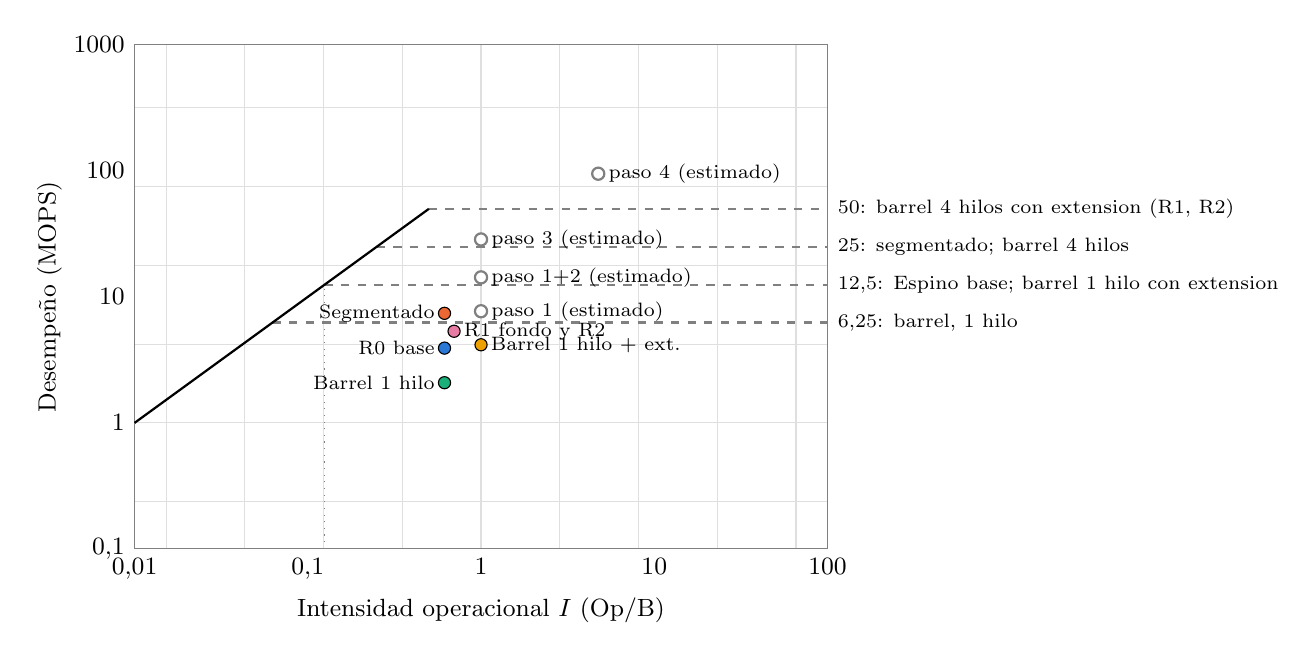
\begin{tikzpicture}[x=2.2cm,y=1.6cm,font=\small]
  \draw[gray!25] (-2,-1) grid (2,3);
  \draw[gray] (-2,-1) rectangle (2,3);
  \node[below] at (-2,-1) {$0{,}01$};
  \node[below] at (-1,-1) {$0{,}1$};
  \node[below] at (0,-1) {$1$};
  \node[below] at (1,-1) {$10$};
  \node[below] at (2,-1) {$100$};
  \node[left] at (-2,-1) {$0{,}1$};
  \node[left] at (-2,0) {$1$};
  \node[left] at (-2,1) {$10$};
  \node[left] at (-2,2) {$100$};
  \node[left] at (-2,3) {$1000$};
  \node[below=5mm] at (0.0,-1) {Intensidad operacional $I$ (Op/B)};
  \node[rotate=90,above=8mm] at (-2,1.0) {Desempeño (MOPS)};
  \draw[gray,dashed,thick] (-1.2041,0.7959) -- (2,0.7959) node[right,black,font=\scriptsize] {6{,}25: barrel{,} 1 hilo};
  \draw[gray,dashed,thick] (-0.9031,1.0969) -- (2,1.0969) node[right,black,font=\scriptsize] {12{,}5: Espino base; barrel 1 hilo con extension};
  \draw[gray,dashed,thick] (-0.6021,1.3979) -- (2,1.3979) node[right,black,font=\scriptsize] {25: segmentado; barrel 4 hilos};
  \draw[gray,dashed,thick] (-0.3010,1.6990) -- (2,1.6990) node[right,black,font=\scriptsize] {50: barrel 4 hilos con extension (R1{,} R2)};
  \draw[black,thick] (-2,0.0000) -- (-0.3010,1.6990);
  \draw[gray,dotted] (-0.9031,-1) -- (-0.9031,1.0969);
  \filldraw[fill={rgb,255:red,42;green,120;blue,214}] (-0.2108,0.5935) circle (2.2pt) node[left,font=\scriptsize,black] {R0 base};
  \filldraw[fill={rgb,255:red,235;green,104;blue,52}] (-0.2108,0.8697) circle (2.2pt) node[left,font=\scriptsize,black] {Segmentado};
  \filldraw[fill={rgb,255:red,27;green,175;blue,122}] (-0.2108,0.3188) circle (2.2pt) node[left,font=\scriptsize,black] {Barrel 1 hilo};
  \filldraw[fill={rgb,255:red,237;green,161;blue,0}] (0.0000,0.6198) circle (2.2pt) node[right,font=\scriptsize,black] {Barrel 1 hilo + ext.};
  \filldraw[fill={rgb,255:red,232;green,123;blue,164}] (-0.1556,0.7272) circle (2.2pt) node[right,font=\scriptsize,black] {R1 fondo y R2};
  \filldraw[draw=gray,thick,fill=white] (0.0000,0.8861) circle (2.2pt) node[right,font=\scriptsize,black] {paso 1 (estimado)};
  \filldraw[draw=gray,thick,fill=white] (0.0000,1.1549) circle (2.2pt) node[right,font=\scriptsize,black] {paso 1+2 (estimado)};
  \filldraw[draw=gray,thick,fill=white] (0.0000,1.4559) circle (2.2pt) node[right,font=\scriptsize,black] {paso 3 (estimado)};
  \filldraw[draw=gray,thick,fill=white] (0.6767,1.9777) circle (2.2pt) node[right,font=\scriptsize,black] {paso 4 (estimado)};
\end{tikzpicture}
